\documentclass{beamer}
\usetheme{Madrid} % 使用Madrid主题,与BIGAI模板布局更匹配
\usecolortheme{default} % 使用默认颜色,然后自定义

\usepackage[utf8]{inputenc}
\usepackage{amsmath}
\usepackage{amsfonts}
\usepackage{amssymb}
\usepackage{graphicx} % For including images
\usepackage{booktabs} % For better tables
\usepackage{hyperref} % For clickable links

% 简化的颜色方案,减少颜色种类
\definecolor{BigAIBlue}{RGB}{0,102,204}  % 主蓝色
\definecolor{BigAIGray}{RGB}{102,102,102}  % 中性灰
\definecolor{BigAILightGray}{RGB}{248,248,248}  % 极浅灰

% 设置简化的颜色主题
\setbeamercolor{structure}{fg=BigAIBlue}
\setbeamercolor{title}{fg=white,bg=BigAIBlue}
\setbeamercolor{frametitle}{fg=BigAIBlue,bg=white}
\setbeamercolor{normal text}{fg=black,bg=white}
\setbeamercolor{alerted text}{fg=BigAIBlue}
\setbeamercolor{block title}{fg=white,bg=BigAIBlue}
\setbeamercolor{block body}{fg=black,bg=BigAILightGray}

% 设置页眉页脚颜色(简化)
\setbeamercolor{headline}{fg=white,bg=white}
\setbeamercolor{footline}{fg=BigAIGray,bg=white}

% 设置字体
\setbeamerfont{title}{size=\Large,series=\bfseries}
\setbeamerfont{frametitle}{size=\large,series=\bfseries}
\setbeamerfont{block title}{size=\normalsize,series=\bfseries}

% 自定义页眉,简化设计,不放置logo
\setbeamertemplate{headline}{
  \leavevmode%
  \hbox{%
  \begin{beamercolorbox}[wd=\paperwidth,ht=2ex,dp=0.5ex,leftskip=.3cm,rightskip=.3cm plus1fil]{headline}% Reduced height, icon removed
    \usebeamerfont{title in head/foot}\hfill % 页眉不放置logo,保持简洁
    % Icon removed from headline
  \end{beamercolorbox}%
  }%
  \vskip0pt%
}

% 在标题页添加BIGAI logo(去掉,因为现在在页脚显示)
\titlegraphic{
  \vspace{1cm}
  % 不在这里显示logo了
}

% 自定义页脚,左下角放置icon2,右下角放置页码
\setbeamertemplate{footline}{
  \leavevmode%
  \hbox{%
  \begin{beamercolorbox}[wd=0.5\paperwidth,ht=4.5ex,dp=1ex,left,leftskip=1ex]{footline} % Icon on the left, increased height
    
\includegraphics[height=4ex]{template/BIGAI_icon2.png}%
  \end{beamercolorbox}%
  \begin{beamercolorbox}[wd=0.5\paperwidth,ht=4.5ex,dp=1ex,right,rightskip=1ex]{footline} % Page number on the right, increased height
    \usebeamerfont{page number in head/foot}\insertframenumber{} / \inserttotalframenumber%
  \end{beamercolorbox}%
  }%
  \vskip0pt%
}

% Bibliography setup
\usepackage[style=authoryear-comp,natbib=true,backend=biber,maxcitenames=2,maxbibnames=99]{biblatex}
\addbibresource{references.bib}

% 自定义引用格式
\renewcommand*{\nameyeardelim}{\addcomma\space}

% 自定义脚注引用命令
\newcommand{\fcite}[1]{\cite{#1}\footnote{\tiny\fullcite{#1}}}

% 增强的视觉设置(简化版)
\setbeamertemplate{blocks}[rounded][shadow=false]  % 去掉阴影,更简约
\setbeamertemplate{itemize items}[circle]
\setbeamercolor{itemize item}{fg=BigAIBlue}
\setbeamercolor{itemize subitem}{fg=BigAIGray}  % 使用灰色而不是蓝色

% 移除默认导航符号
\setbeamertemplate{navigation symbols}{}

% 自定义标题页设计,匹配简约风格
\setbeamertemplate{title page}{
  \vbox{}
  \vfill
  \begingroup
    \centering
    \begin{beamercolorbox}[sep=8pt,center,colsep=-4bp,rounded=true,shadow=false]{title}
      \usebeamerfont{title}\inserttitle\par%
      \ifx\insertsubtitle\@empty%
      \else%
        \vskip0.25em%
        {\usebeamerfont{subtitle}\usebeamercolor[fg]{subtitle}\insertsubtitle\par}%
      \fi%     
    \end{beamercolorbox}%
    \vskip1em\par
    \begin{beamercolorbox}[sep=8pt,center,colsep=-4bp,rounded=true]{author}
      \usebeamerfont{author}\insertauthor
    \end{beamercolorbox}
    \begin{beamercolorbox}[sep=8pt,center,colsep=-4bp,rounded=true]{institute}
      \usebeamerfont{institute}\insertinstitute
    \end{beamercolorbox}
    \begin{beamercolorbox}[sep=8pt,center,colsep=-4bp,rounded=true]{date}
      \usebeamerfont{date}\insertdate
    \end{beamercolorbox}\vskip0.5em
    {\usebeamercolor[fg]{titlegraphic}\inserttitlegraphic\par}
  \endgroup
  \vfill
}

\title[MoE \& Tokenization in Deep RL]{Breaking the Parameter Scaling Barrier in Deep RL: The Power of Soft Mixtures of Experts and Tokenization}
\author[Research Presentation]{Based on \fcite{ceron2024mixtures} and \fcite{sokar2024tokenize}}
\institute{Beijing Institute for General Artificial Intelligence (BIGAI)}
\date{\today}

\begin{document}

% --- Title Page ---
\begin{frame}
  \titlepage
\end{frame}

% --- Outline ---
\begin{frame}{Research Overview}
  \begin{center}
    \Large \textbf{Two Groundbreaking Studies, One Revolutionary Insight}
  \end{center}
  
  \vspace{0.5em}
  \begin{columns}[T]
    \begin{column}{0.48\textwidth}
      \begin{block}{Paper 1: Ceron et al. (2024)}
        \small
        \textbf{Finding:} SoftMoE enables parameter scaling\\
        \textbf{Question:} Why does it work?
        \begin{itemize}
          \item[\checkmark] Proved scaling is possible
          \item[\checkmark] Showed consistent improvements
          \item[?] Mechanism unclear
        \end{itemize}
      \end{block}
    \end{column}
    \begin{column}{0.48\textwidth}
      \begin{block}{Paper 2: Sokar et al. (2024)}
        \small
        \textbf{Finding:} Tokenization is the key\\
        \textbf{Answer:} It's not about experts!
        \begin{itemize}
          \item[\checkmark] Isolated the mechanism
          \item[\checkmark] Single expert works
          \item[\checkmark] Tokenization critical
        \end{itemize}
      \end{block}
    \end{column}
  \end{columns}
  
  \vspace{1em}
  \begin{center}
    \colorbox{blue!20}{\parbox{0.8\textwidth}{\centering
    \textbf{Combined Insight:} The secret is not multiple experts,\\
    but how we structure the data flow through tokenization}}
  \end{center}
\end{frame}

% --- Section 1: The Problem ---
\section{Problem Background: Deep RL Scaling Challenges}

\begin{frame}{The Parameter Scaling Problem in Deep RL}
  \begin{columns}[T]
    \begin{column}{0.6\textwidth}
      \begin{figure}
        \centering
        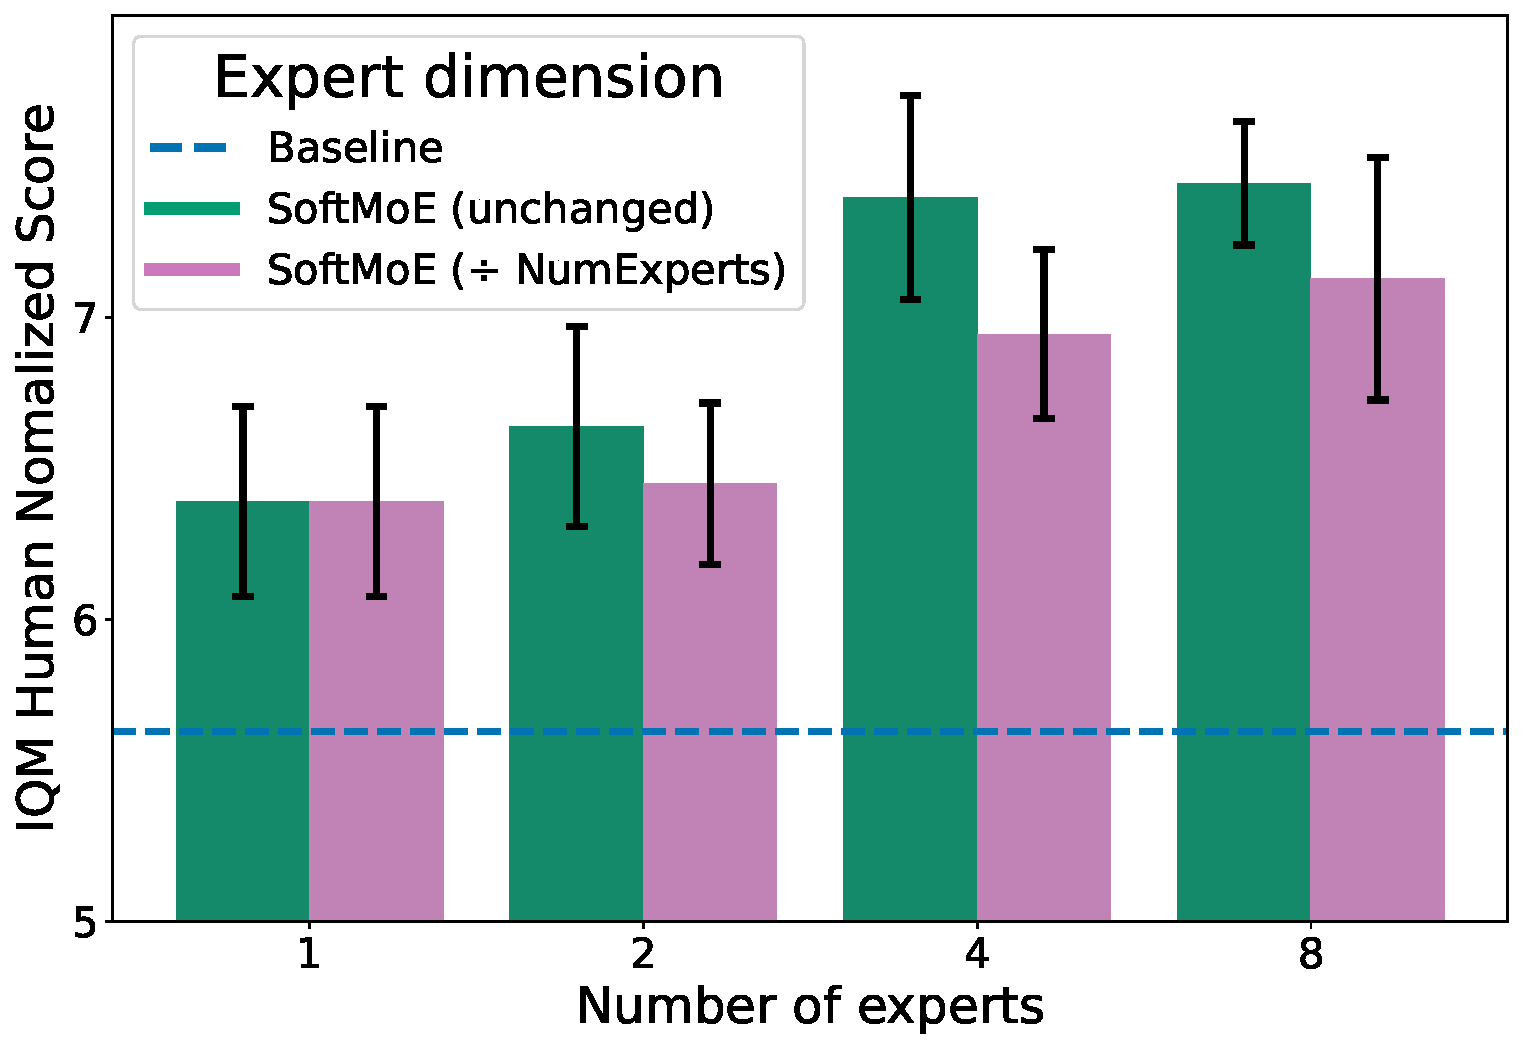
\includegraphics[width=\textwidth]{Mixtures_of_Experts_Unlock Parameter_Scaling_for_Deep_RL/figures/rainbowScalingPlot.pdf}
        \caption{Traditional approach hurts performance}
      \end{figure}
    \end{column}
    \begin{column}{0.4\textwidth}
      \textbf{Key Challenges:}
      \begin{itemize}
        \item Adding parameters \textbf{hurts} RL performance \fcite{ceron2024mixtures}
        \item Difficult to develop scaling laws \fcite{kaplan2020scaling}
        \item Need new architectural approaches
      \end{itemize}
    \end{column}
  \end{columns}
\end{frame}

\begin{frame}{Why Traditional Scaling Methods Fail}
  \begin{columns}[T]
    \begin{column}{0.6\textwidth}
      \begin{figure}
        \centering
        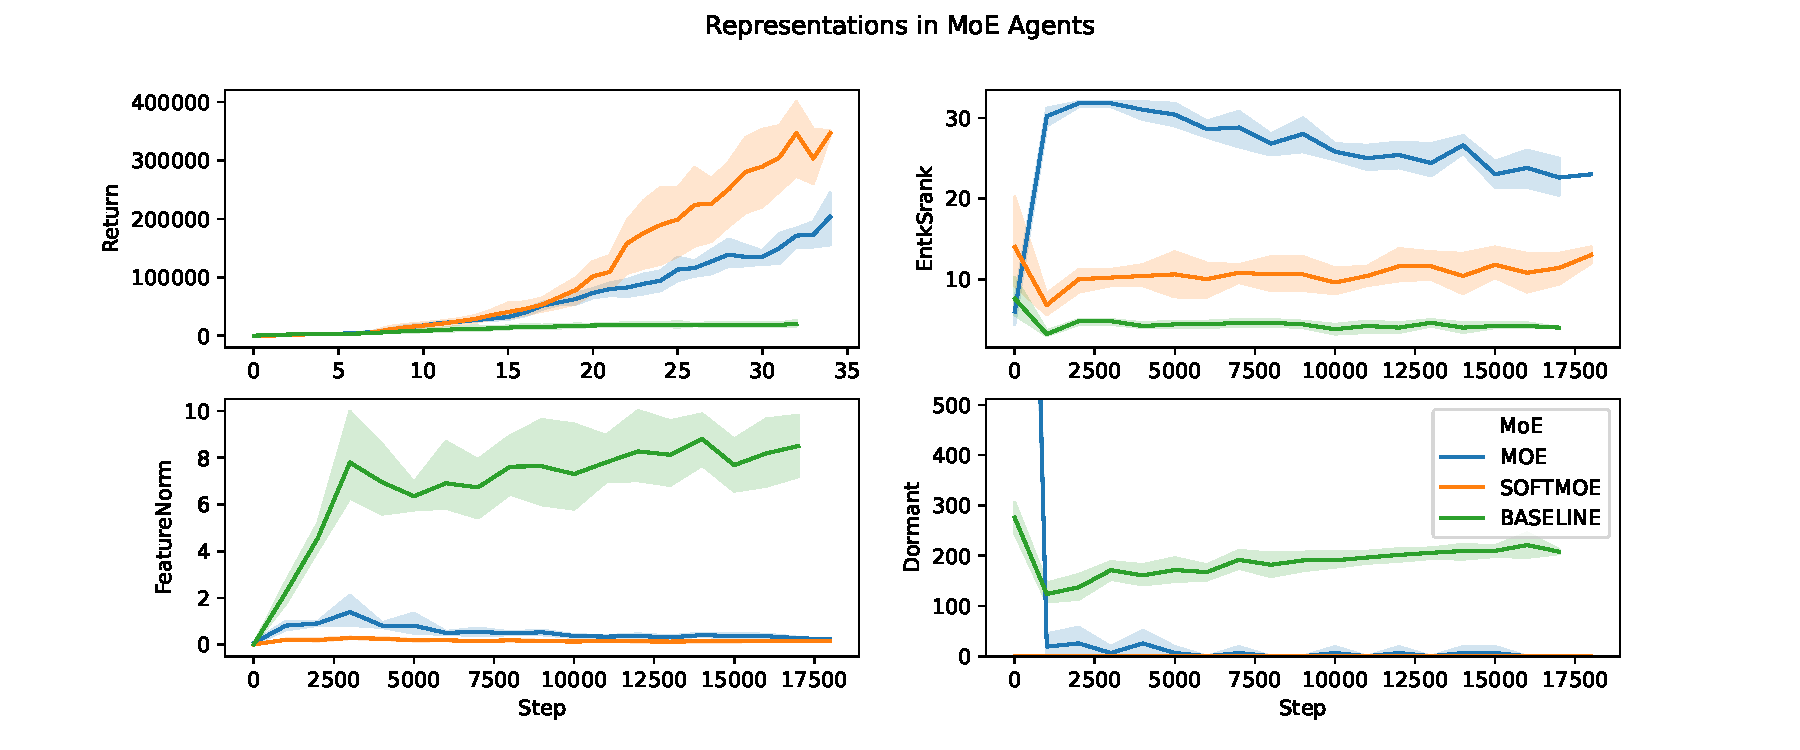
\includegraphics[width=\textwidth]{Mixtures_of_Experts_Unlock Parameter_Scaling_for_Deep_RL/figures/representations.pdf}
        \caption{Unique phenomena in deep RL}
      \end{figure}
    \end{column}
    \begin{column}{0.4\textwidth}
      \textbf{Key Challenges:}
      \begin{itemize}
        \item Dormant neurons \fcite{sokar2023dormant}
        \item Passive learning difficulties
        \item Capacity loss issues
        \item Regularization needs \fcite{kumar2021dr3}
      \end{itemize}
    \end{column}
  \end{columns}
\end{frame}

% --- Section 2: Solution 1 - SoftMoE ---
\section{Solution Exploration: Soft Mixture of Experts}

\begin{frame}{Soft Mixture of Experts (SoftMoE) Architecture}
  \begin{columns}[T]
    \begin{column}{0.55\textwidth}
      \begin{figure}
        \centering
        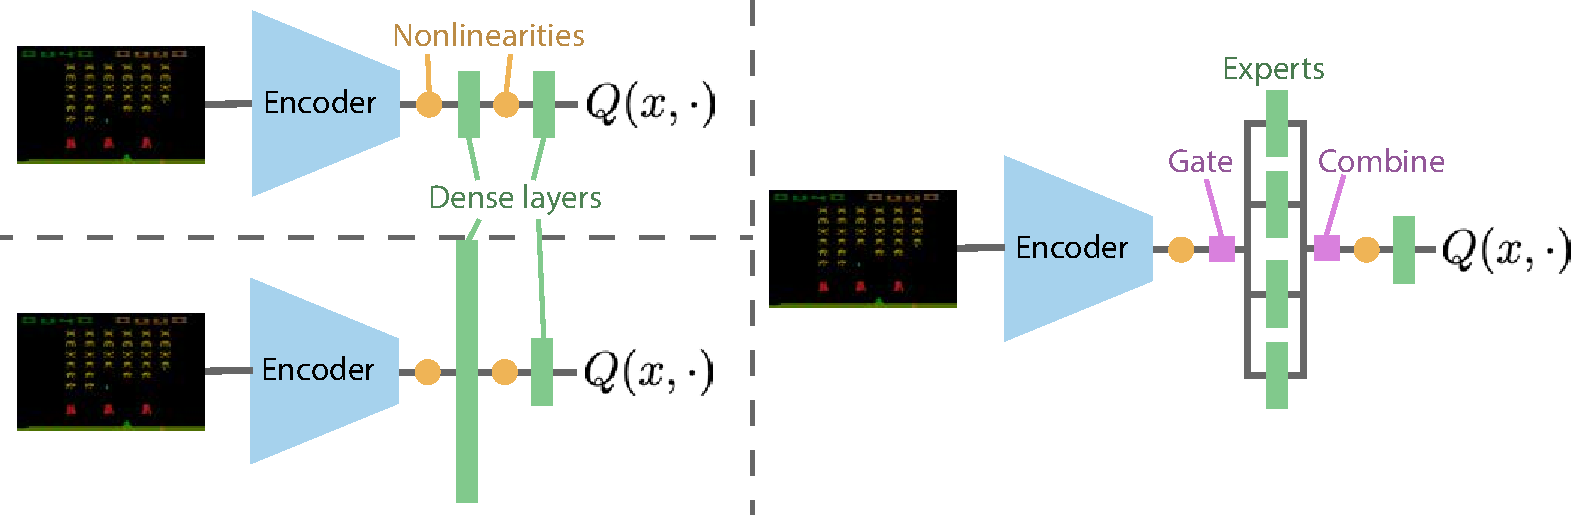
\includegraphics[width=\textwidth]{Mixtures_of_Experts_Unlock Parameter_Scaling_for_Deep_RL/figures/moeArchitecture.pdf}
        \caption{SoftMoE integration in deep RL}
      \end{figure}
    \end{column}
    \begin{column}{0.45\textwidth}
      \textbf{Key Features:}
      \begin{itemize}
        \item \textbf{Soft Assignment}: Differentiable routing
        \item \textbf{Strategic Placement}: Replaces dense layer
        \item \textbf{Spatial Preservation}: Maintains structure
        \item No discrete routing decisions
        \item Fully end-to-end trainable
        \item Computationally efficient
      \end{itemize}
    \end{column}
  \end{columns}
\end{frame}

\begin{frame}{SoftMoE's Breakthrough Results}
  \begin{columns}[T]
    \begin{column}{0.65\textwidth}
      \begin{figure}
        \centering
        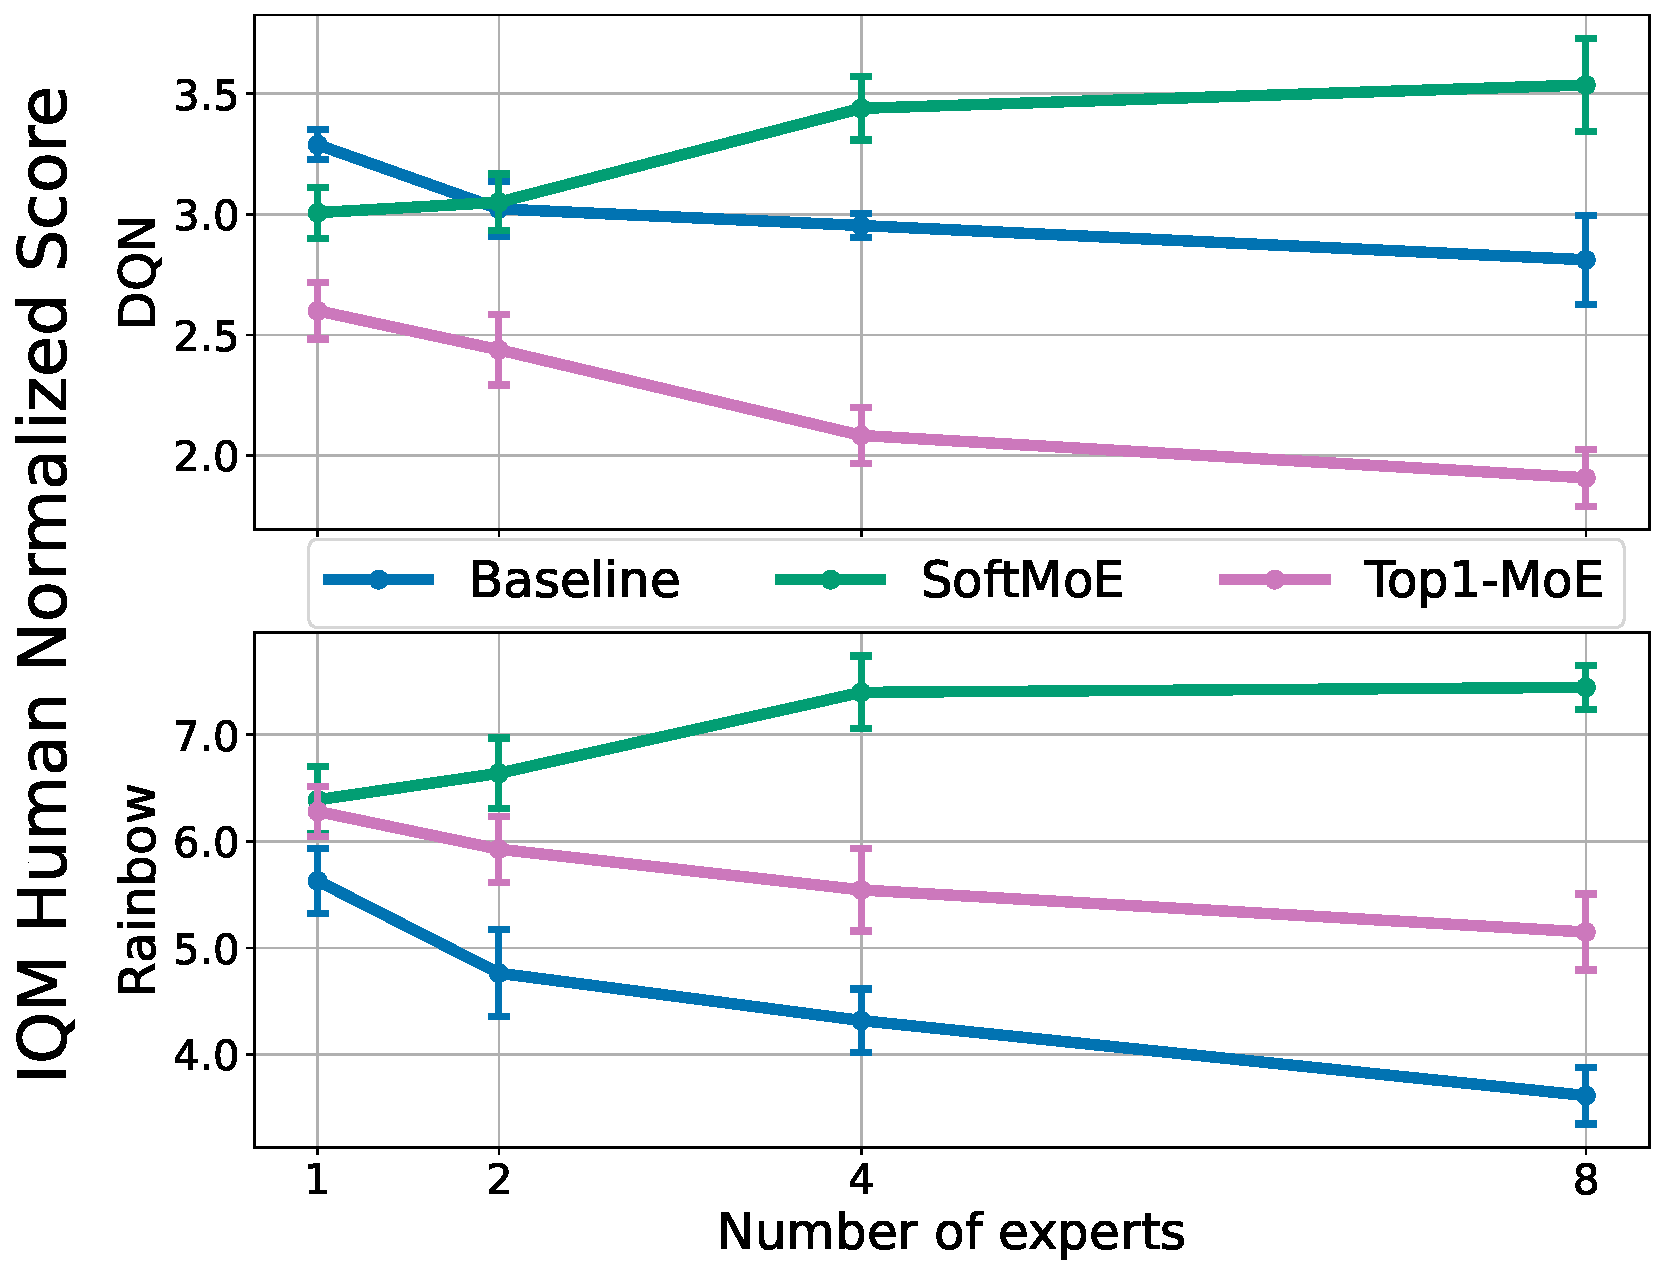
\includegraphics[width=\textwidth]{Mixtures_of_Experts_Unlock Parameter_Scaling_for_Deep_RL/figures/combinedTopline.pdf}
        \caption{SoftMoE achieves parameter scalability}
      \end{figure}
    \end{column}
    \begin{column}{0.35\textwidth}
      \textbf{Key Results:}
      \begin{itemize}
        \item \textbf{20\%} improvement with 8 experts
        \item \textbf{40\%} degradation with traditional scaling
        \item Robust across different settings \fcite{ceron2024mixtures}
      \end{itemize}
    \end{column}
  \end{columns}
\end{frame}

% --- Section 3: Key Discovery - Tokenization ---
\section{Key Discovery: The True Role of Tokenization}

\begin{frame}{Tokenization Scheme Comparison}
  \begin{figure}
    \centering
    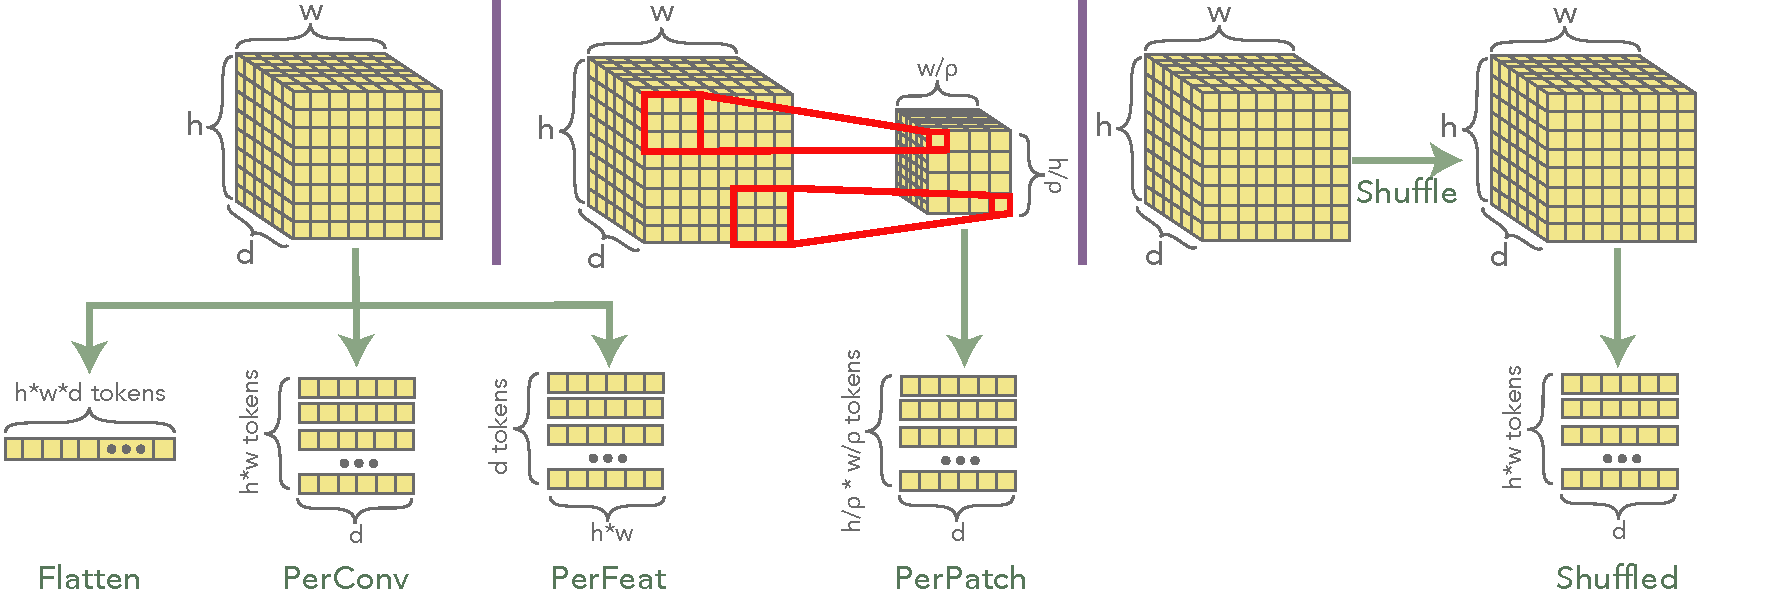
\includegraphics[width=0.8\textwidth]{Don_t_flatten_tokenize/figures/tokenizationSchemes.pdf}
    \caption{Architectural comparison of different tokenization strategies}
  \end{figure}
  
  \begin{itemize}
    \item \textbf{PerConv}: $(h,w,d) \rightarrow h \times w$ tokens of dimension $d$
    \item \textbf{PerFeat}: $(h,w,d) \rightarrow d$ tokens of dimension $h \times w$
    \item \textbf{PerSamp}: Entire output as single token
  \end{itemize}
\end{frame}

\begin{frame}{Surprising Discovery: Single Expert Can Succeed}
  \begin{center}
    \Large \colorbox{red!20}{\textbf{SHOCKING REVELATION}}
  \end{center}
  
  \begin{columns}[T]
    \begin{column}{0.6\textwidth}
      \begin{figure}
        \centering
        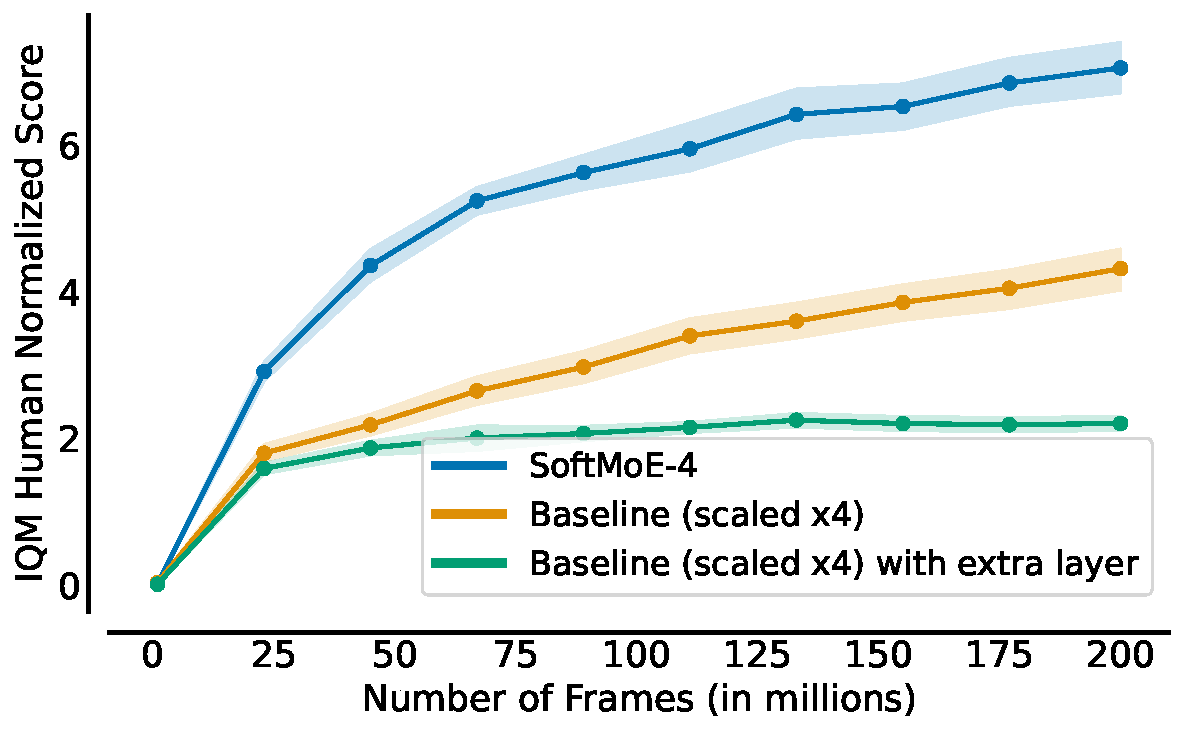
\includegraphics[width=\textwidth]{Don_t_flatten_tokenize/figures/results/SoftMoE-x4_vs_Baseline_w_extralayer.pdf}
        \caption{Single expert vs multi-expert comparison}
      \end{figure}
    \end{column}
    \begin{column}{0.4\textwidth}
      \begin{block}{Core Insight}
        \textbf{Tokenization}, not multiple experts, drives SoftMoE's success!
        
        \vspace{0.5em}
        This challenges the assumption that expert diversity drives performance.
      \end{block}
    \end{column}
  \end{columns}
\end{frame}

\begin{frame}{Tokenization Effectiveness Validation}
  \begin{columns}[T]
    \begin{column}{0.5\textwidth}
      \begin{figure}
        \centering
        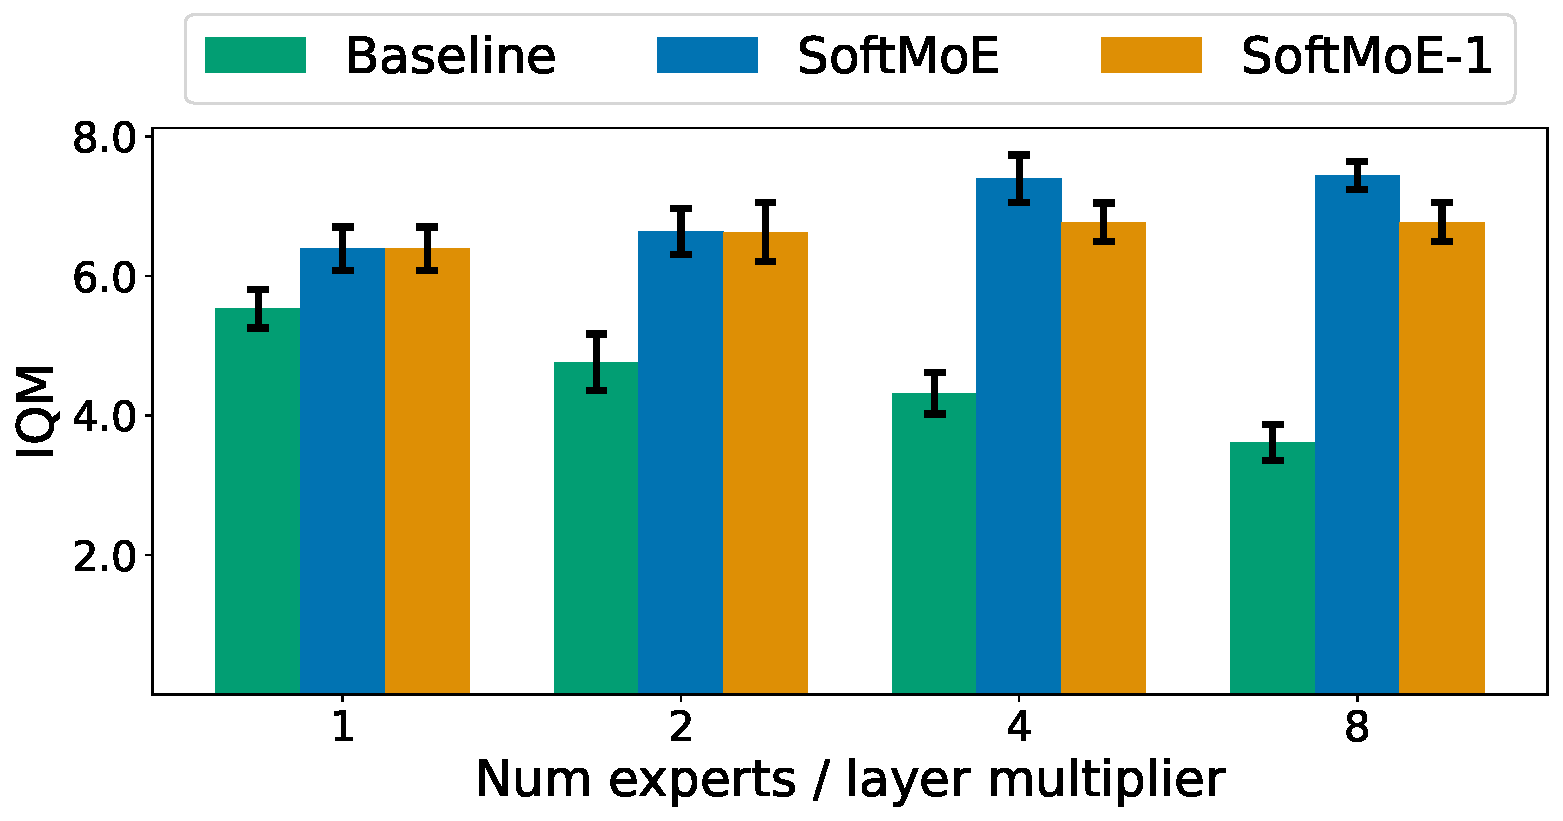
\includegraphics[width=\textwidth]{Don_t_flatten_tokenize/figures/results/aggregate_comparison_just_iqm_bar.pdf}
        \caption{Tokenized baseline vs traditional baseline}
      \end{figure}
    \end{column}
    \begin{column}{0.5\textwidth}
      \begin{figure}
        \centering
        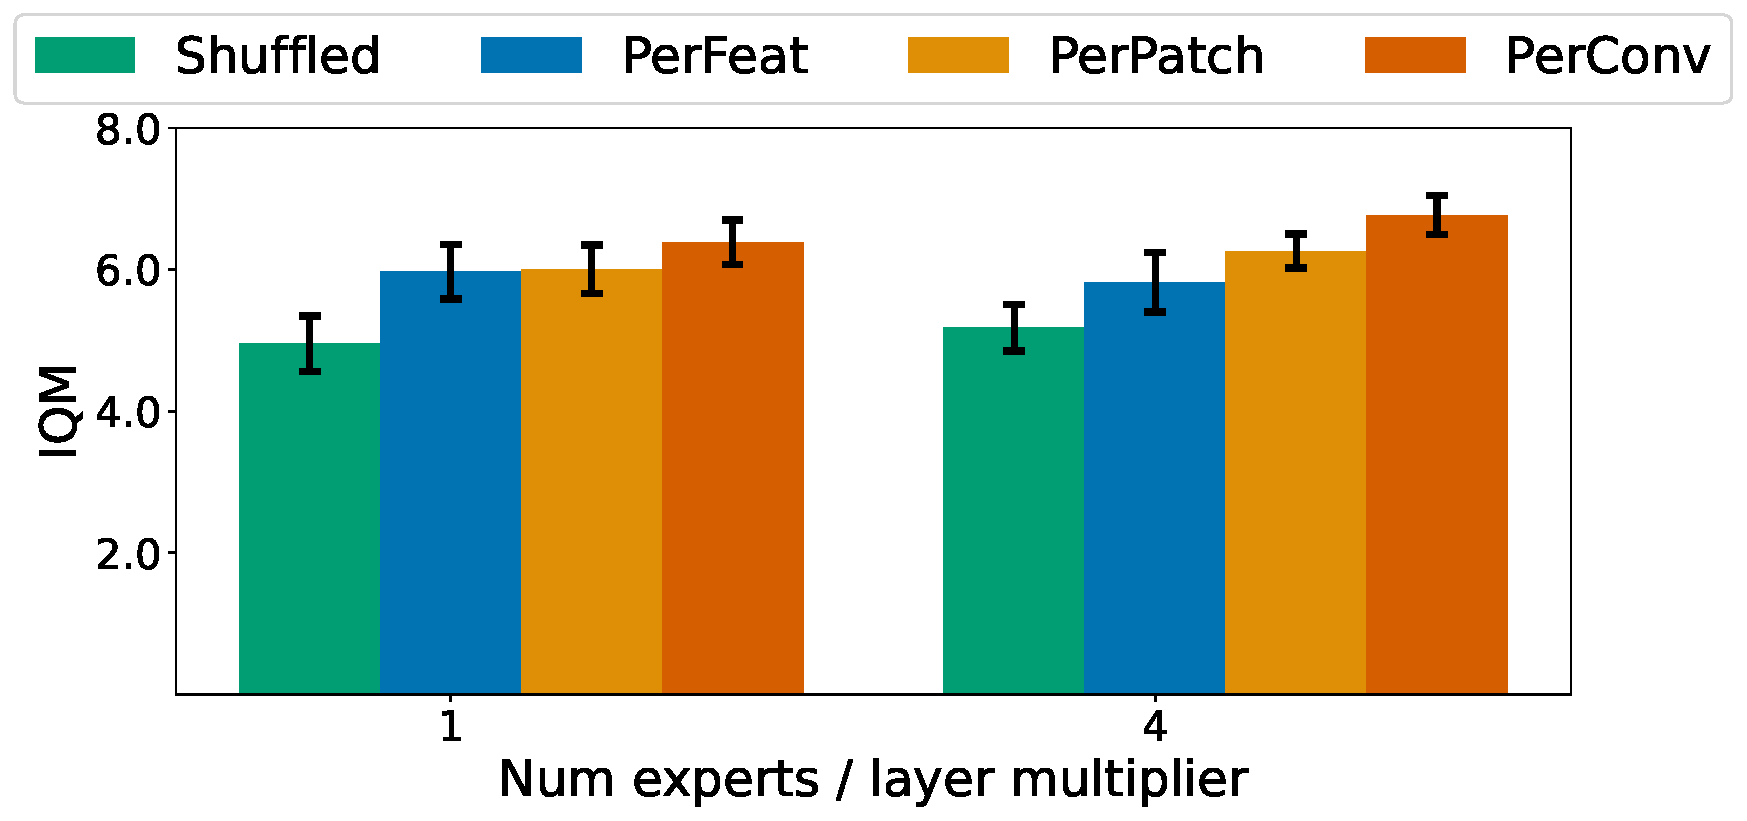
\includegraphics[width=\textwidth]{Don_t_flatten_tokenize/figures/results/tokentypes__just_iqm_bar.pdf}
        \caption{Effects of different tokenization schemes}
      \end{figure}
    \end{column}
  \end{columns}
  
  \begin{itemize}
    \item Simple tokenized baseline significantly improves performance
    \item PerConv tokenization works best
    \item Preserving spatial structure is crucial
  \end{itemize}
\end{frame}

% --- Section 4: Architecture Analysis ---
\section{Deep Analysis: Architecture Comparison \& Mechanism}

\begin{frame}{Architecture Comparison: Traditional vs Tokenized}
  \begin{figure}
    \centering
    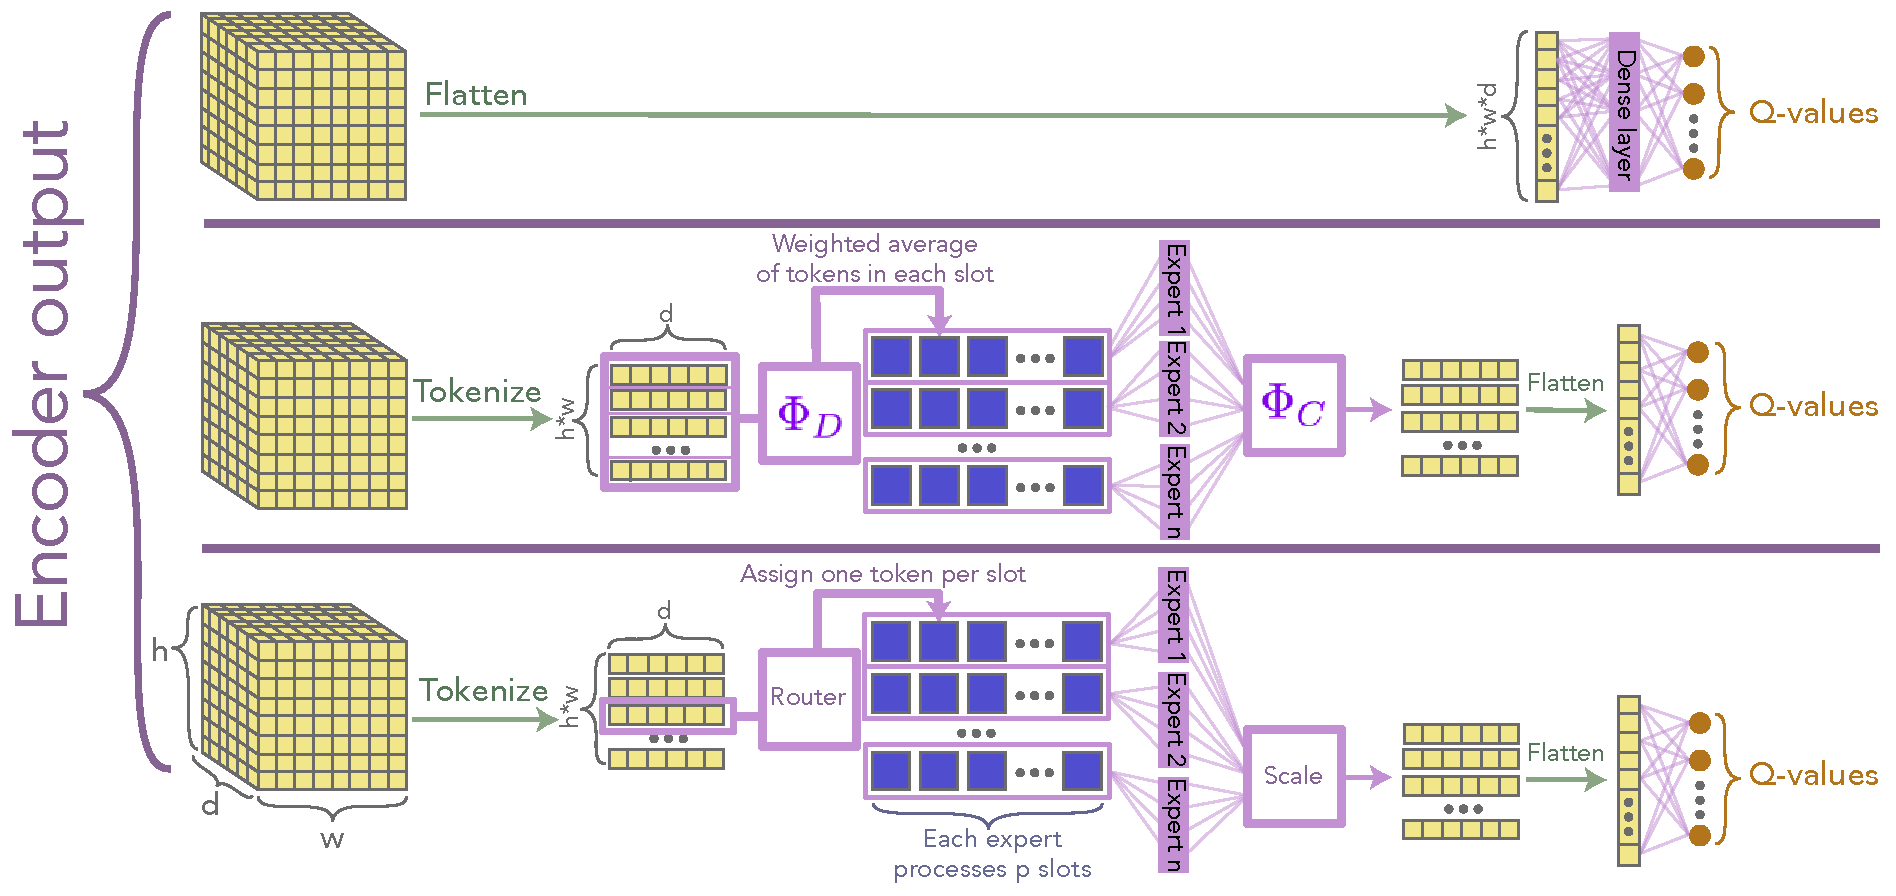
\includegraphics[width=0.9\textwidth]{Don_t_flatten_tokenize/figures/architectures.pdf}
    \caption{Baseline, SoftMoE, and Top-k MoE architecture comparison}
  \end{figure}
  
  \begin{itemize}
    \item \textbf{Traditional approach}: Flattens encoder output
    \item \textbf{MoE approach}: Tokenizes then processes by experts
    \item \textbf{Key difference}: Preserving vs losing spatial information
  \end{itemize}
\end{frame}

\begin{frame}{Expert Utilization Analysis: The Redundancy Problem}
  \begin{columns}[T]
    \begin{column}{0.5\textwidth}
      \begin{figure}
        \centering
        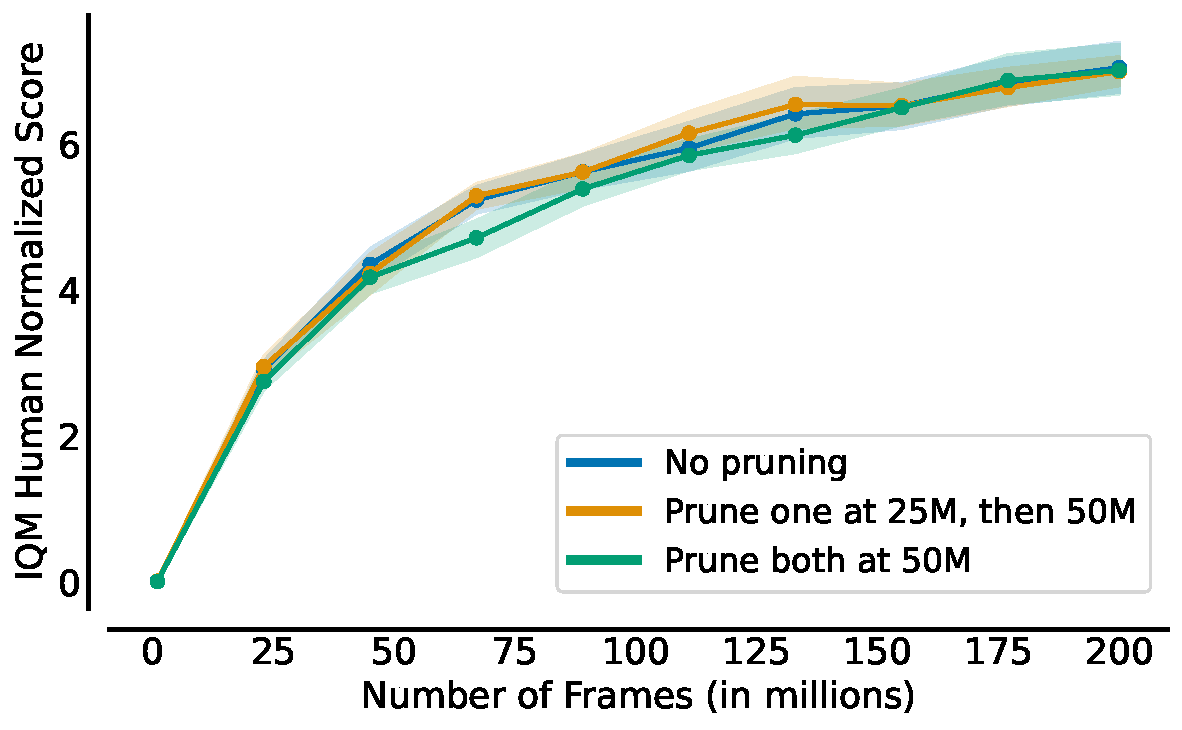
\includegraphics[width=\textwidth]{Don_t_flatten_tokenize/figures/results/SoftMoE-4-ExpertsPruning.pdf}
        \caption{Expert pruning experiment}
      \end{figure}
    \end{column}
    \begin{column}{0.5\textwidth}
      \begin{block}{Pruning Test Results}
        \small
        Remove 50\% of experts:
        \begin{itemize}
          \item Performance drop: \textcolor{red}{\textbf{$< 2\%$}}
          \item Training: \textcolor{green}{\textbf{Stable}}
          \item Convergence: \textcolor{green}{\textbf{Unchanged}}
        \end{itemize}
      \end{block}
      
      \vspace{0.3em}
      \begin{block}{Implications}
        \small
        \begin{itemize}
          \item Experts learn similar representations
          \item Scaling experts $\neq$ Scaling performance
          \item Tokenization does the heavy lifting
        \end{itemize}
      \end{block}
    \end{column}
  \end{columns}
  
  \vspace{0.5em}
  \begin{center}
    \colorbox{yellow!30}{\parbox{0.9\textwidth}{\centering
    \textbf{Paradigm Shift:} Focus on tokenization design, not expert architecture}}
  \end{center}
\end{frame}

% --- Section 5: Broader Applications ---
\section{Extended Applications \& Real Impact}

\begin{frame}{Cross-Algorithm Effectiveness}
  \begin{columns}[T]
    \begin{column}{0.5\textwidth}
      \begin{figure}
        \centering
        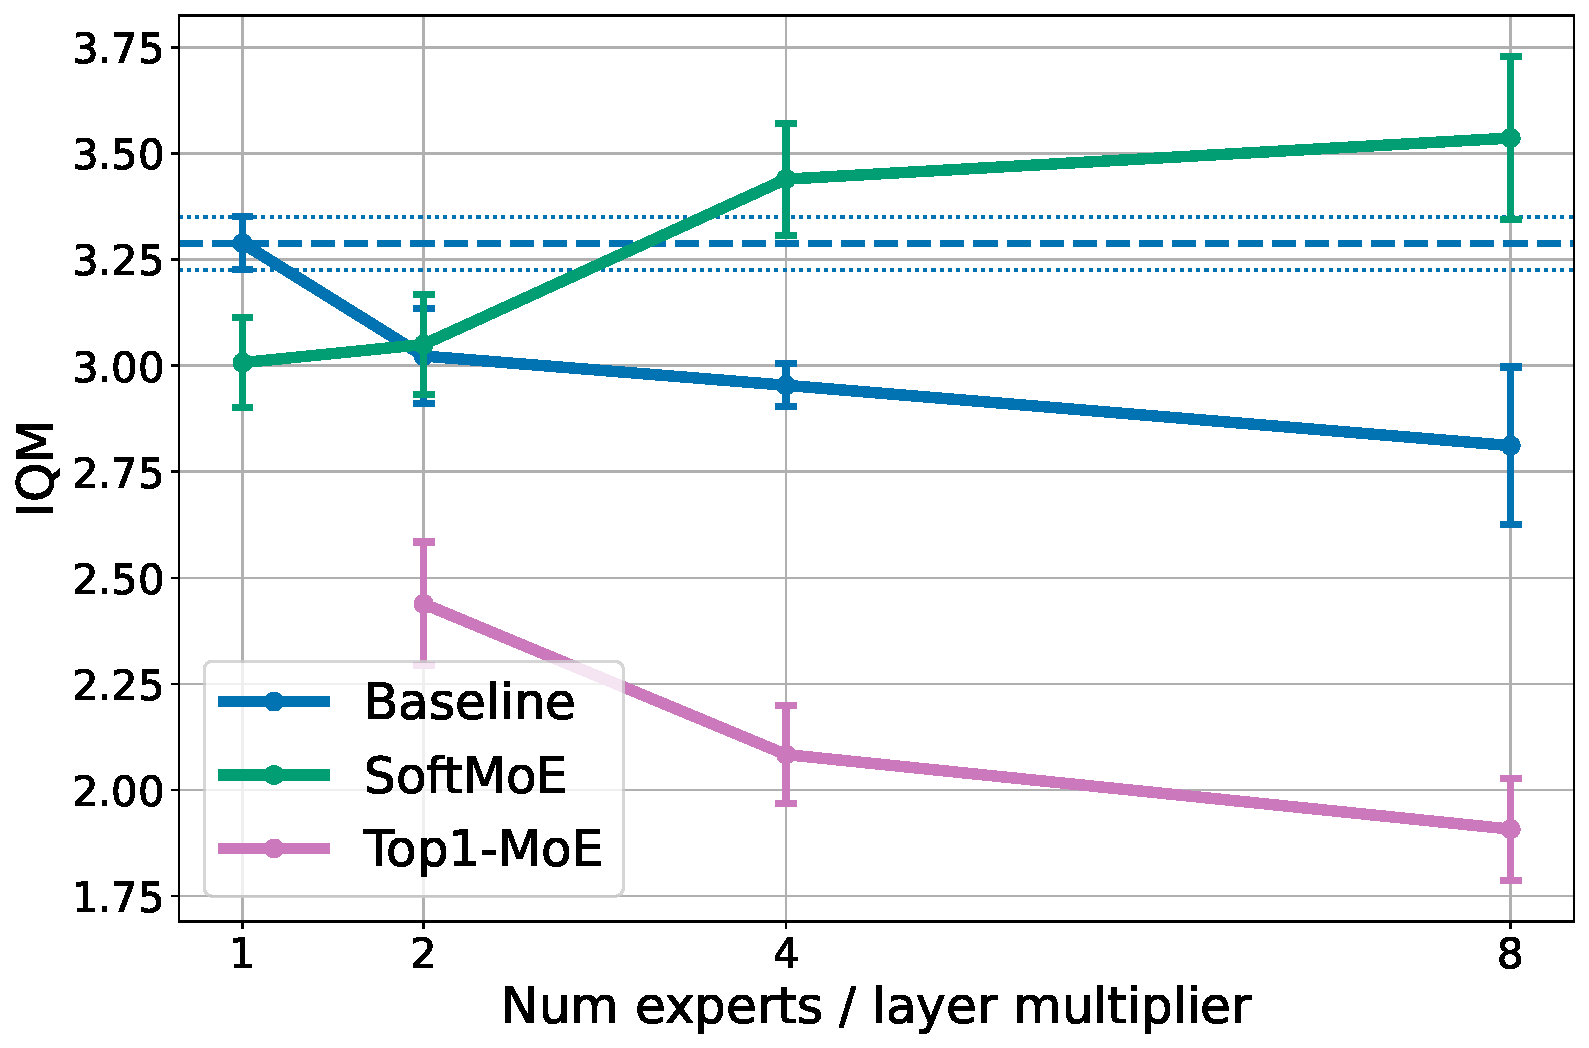
\includegraphics[width=\textwidth]{Mixtures_of_Experts_Unlock Parameter_Scaling_for_Deep_RL/figures/dqnToplinePlot.pdf}
        \caption{DQN algorithm results}
      \end{figure}
    \end{column}
    \begin{column}{0.5\textwidth}
      \begin{figure}
        \centering
        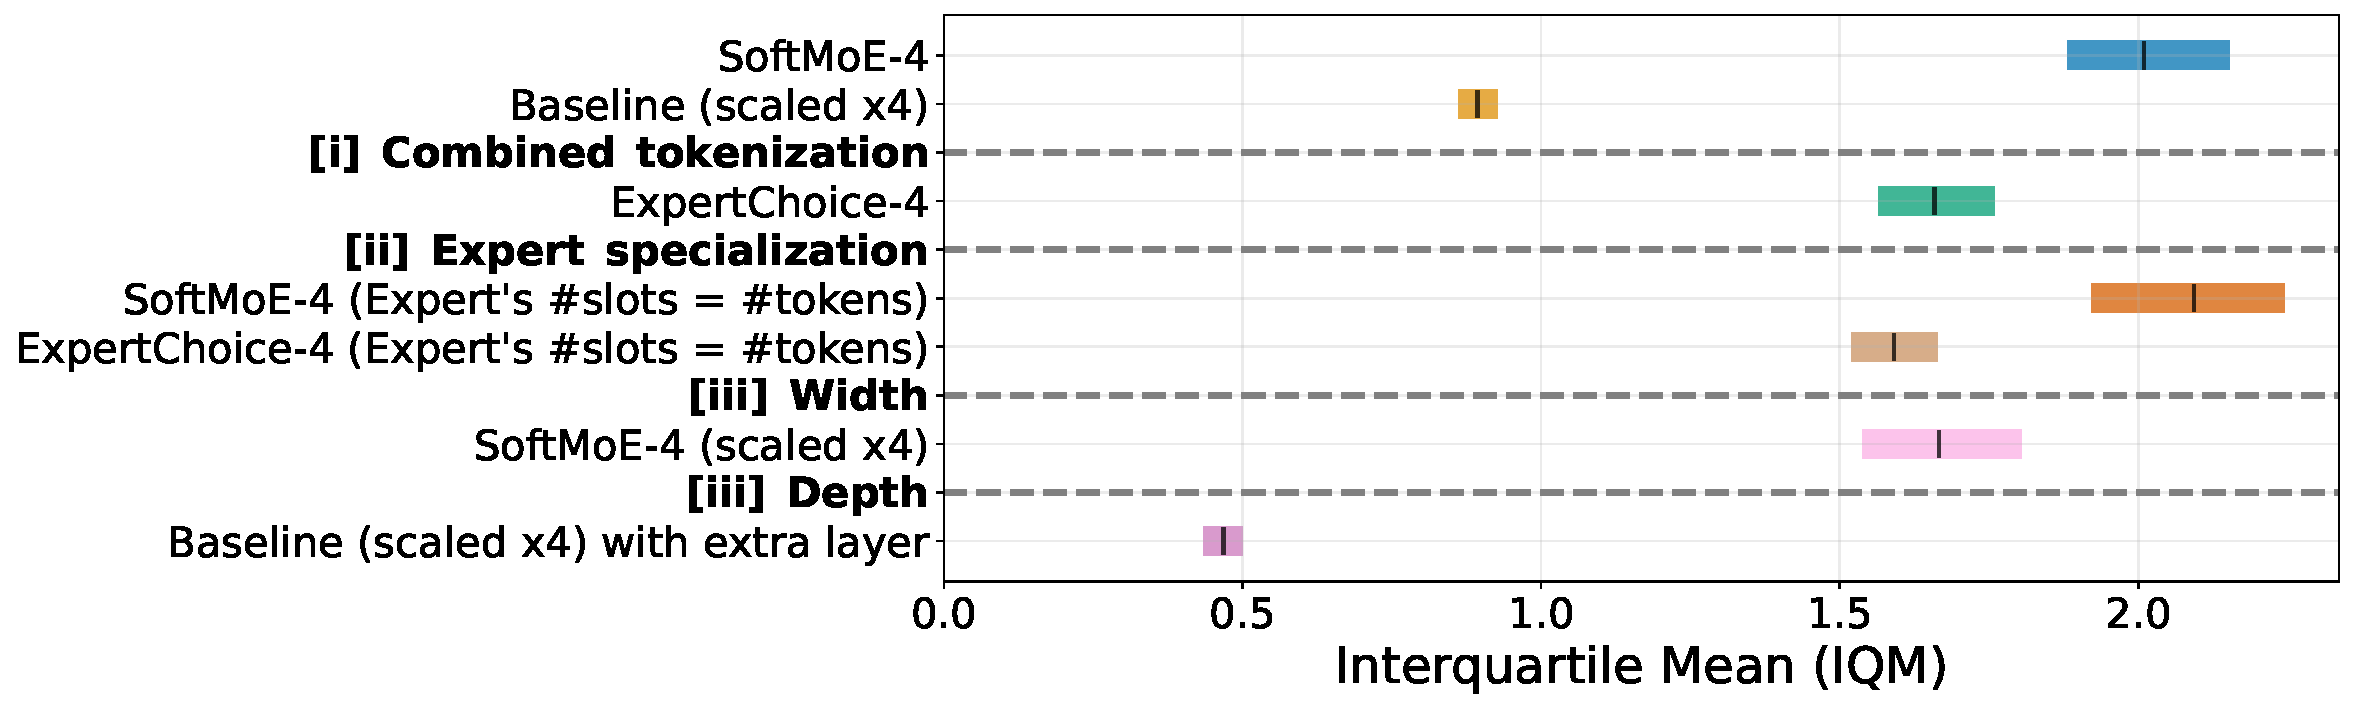
\includegraphics[width=\textwidth]{Don_t_flatten_tokenize/figures/results/section4_DER_aggregate_v2.pdf}
        \caption{DER algorithm results}
      \end{figure}
    \end{column}
  \end{columns}
  
  \begin{itemize}
    \item \textbf{DQN}: Basic value function learning
    \item \textbf{Rainbow}: Combination of multiple improvements
    \item \textbf{DER}: Data efficiency regularization method
    \item Tokenization shows improvements across different algorithms
  \end{itemize}
\end{frame}

\begin{frame}{Network Architecture Generality}
  \begin{columns}[T]
    \begin{column}{0.5\textwidth}
      \begin{figure}
        \centering
        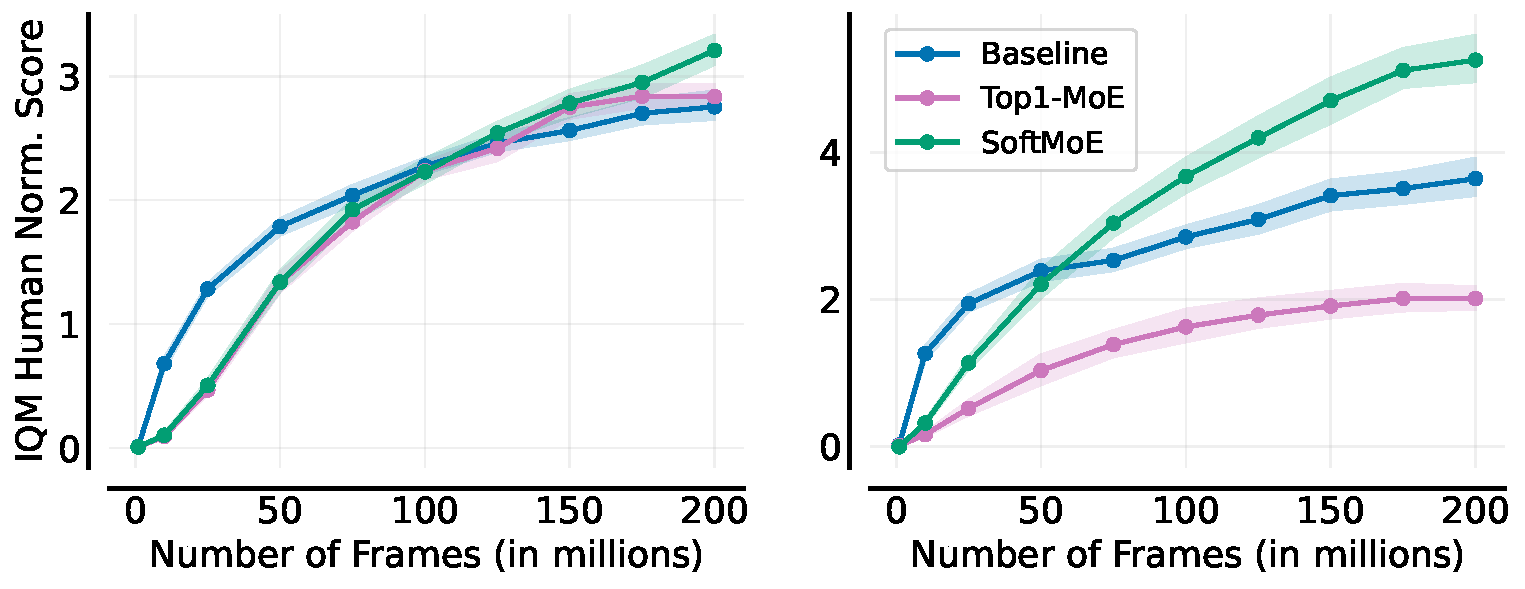
\includegraphics[width=\textwidth]{Mixtures_of_Experts_Unlock Parameter_Scaling_for_Deep_RL/figures/combinedCNN.pdf}
        \caption{CNN encoder results}
      \end{figure}
    \end{column}
    \begin{column}{0.5\textwidth}
      \begin{figure}
        \centering
        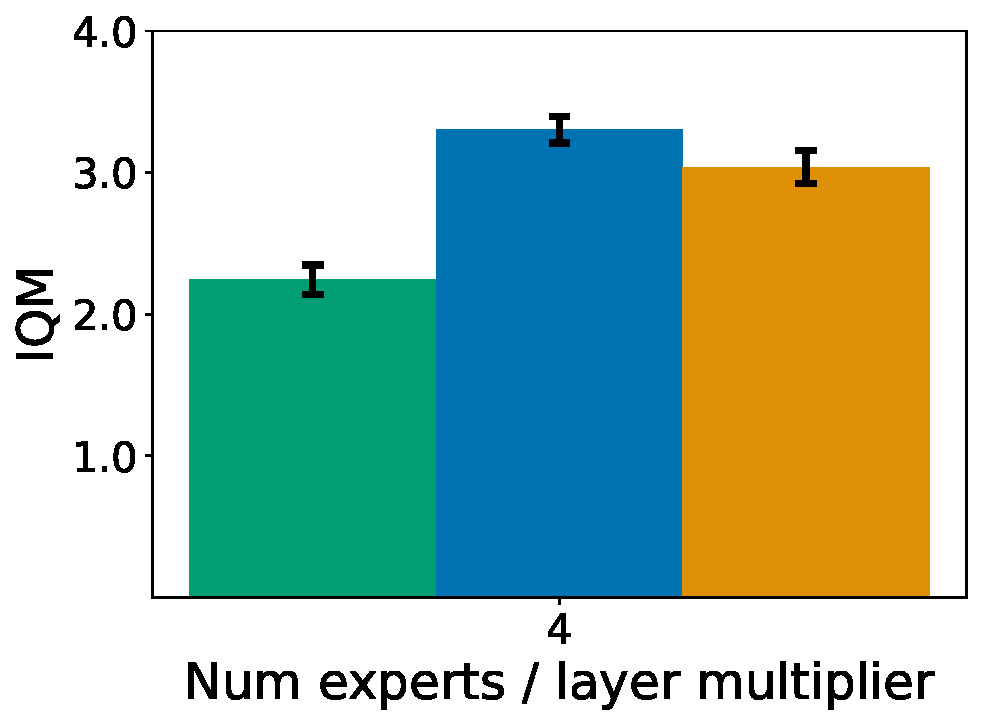
\includegraphics[width=\textwidth]{Don_t_flatten_tokenize/figures/results/60games_aggregate_comparison_just_iqm_bar.pdf}
        \caption{Full 60-game suite results}
      \end{figure}
    \end{column}
  \end{columns}
  
  \begin{itemize}
    \item Works not only with Impala but also standard CNN encoders
    \item Improvements across all 60 Atari games
    \item Method has broad applicability
  \end{itemize}
\end{frame}

% --- Section 6: Implications and Future ---
\section{Important Insights \& Future Directions}

\begin{frame}{Rethinking Deep RL Architecture Design}
  \begin{block}{Core Insights}
    \begin{itemize}
      \item \textbf{Flattening is harmful}: Traditional flattening may lose critical spatial information
      \item \textbf{Tokenization is key}: Spatial structure-preserving tokenization drives performance gains
      \item \textbf{Expert redundancy}: Current MoE setups have low expert utilization
      \item \textbf{Parameter scaling}: Correct architecture design enables effective parameter scaling
    \end{itemize}
  \end{block}
  
  \begin{block}{Design Principles}
    \begin{itemize}
      \item Prioritize spatial information preservation
      \item Explore more effective expert allocation strategies
      \item Reevaluate traditional architectural assumptions
    \end{itemize}
  \end{block}
\end{frame}

\begin{frame}{Future Research Directions}
  \begin{columns}[T]
    \begin{column}{0.5\textwidth}
      \textbf{Architecture Optimization}
      \begin{itemize}
        \item More efficient tokenization schemes
        \item Expert specialization mechanisms
        \item Adaptive routing strategies
        \item Computational efficiency optimization
      \end{itemize}
      
      \textbf{Application Extension}
      \begin{itemize}
        \item Continuous control tasks
        \item Multi-task reinforcement learning
        \item Offline reinforcement learning
        \item Large-scale environments
      \end{itemize}
    \end{column}
    \begin{column}{0.5\textwidth}
      \textbf{Theoretical Understanding}
      \begin{itemize}
        \item Theoretical foundations of tokenization
        \item Expert dynamics analysis
        \item Scaling law research
        \item Generalization capability analysis
      \end{itemize}
      
      \textbf{Practical Deployment}
      \begin{itemize}
        \item Distributed training optimization
        \item Inference efficiency improvement
        \item Hardware adaptation
        \item Industrial applications
      \end{itemize}
    \end{column}
  \end{columns}
\end{frame}

% --- Conclusion ---
\section{Conclusion}

\begin{frame}{Research Summary}
  \begin{center}
    \Large \textbf{Complete Path from Problem to Solution}
  \end{center}
  
  \begin{enumerate}
    \item \textbf{Problem Identification}: Parameter scaling difficulties in deep RL \fcite{ceron2024mixtures}
    \item \textbf{Solution}: SoftMoE achieves parameter scalability
    \item \textbf{Mechanism Discovery}: Tokenization is the key success factor \fcite{sokar2024tokenize}
    \item \textbf{Deep Insights}: Rethinking architectural design paradigms
  \end{enumerate}
  
  \vspace{1em}
  \begin{block}{Main Contributions}
    \begin{itemize}
      \item First effective parameter scaling in deep RL
      \item Revealed tokenization's key role in MoE success
      \item Provided new guidance principles for future architecture design
    \end{itemize}
  \end{block}
\end{frame}

\begin{frame}{Key Takeaways}
  \begin{columns}[T]
    \begin{column}{0.5\textwidth}
      \textbf{What We Learned:}
      \begin{itemize}
        \item Traditional flattening loses spatial information
        \item Tokenization preserves crucial structure
        \item Single expert + tokenization $\approx$ Multi-expert performance
        \item Expert redundancy is a real issue
      \end{itemize}
    \end{column}
    \begin{column}{0.5\textwidth}
      \textbf{Design Guidelines:}
      \begin{itemize}
        \item Preserve spatial structure in conv outputs
        \item Focus on tokenization over expert count
        \item Consider computational efficiency
        \item Evaluate expert utilization
      \end{itemize}
    \end{column}
  \end{columns}
  
  \vspace{1em}
  \begin{center}
    \textbf{The paradigm shift:} From "How many experts?" to "How to tokenize?"
  \end{center}
\end{frame}

\begin{frame}{Impact \& Broader Implications}
  \begin{block}{Immediate Impact}
    \begin{itemize}
      \item Enables parameter scaling in deep RL for the first time
      \item Works across multiple RL algorithms (DQN, Rainbow, DER)
      \item Applicable to different network architectures (CNN, Impala)
      \item Validated on large-scale benchmarks (60 Atari games)
    \end{itemize}
  \end{block}
  
  \begin{block}{Broader Implications}
    \begin{itemize}
      \item Challenges conventional architectural wisdom in RL
      \item Opens new research directions in tokenization schemes
      \item Potential applications beyond visual RL tasks
      \item Foundation for developing RL scaling laws
    \end{itemize}
  \end{block}
\end{frame}

% --- Q&A ---
\begin{frame}
  \begin{center}
    \Huge Thank You!\\
    \vspace{1em}
    \Large Questions \& Discussion
  \end{center}
  
  \vspace{2em}
  \begin{center}
    \textit{Rethinking Deep RL Architecture Design:\\
    From Flattening to Tokenization}
  \end{center}
\end{frame}

\end{document}